% ------------------------------------------------------------------
%  Figura: Ciclo de Auto-Recuperación (slide 17)
%  Compilar:  pdflatex 17_recuperacion.tex
% ------------------------------------------------------------------
\documentclass[tikz, border=0.2cm]{standalone}
\usepackage[utf8]{inputenc}
\usepackage[T1]{fontenc}
\usepackage{libertine}
\usepackage{xcolor}

\definecolor{primary}{HTML}{280091}
\definecolor{secondary}{HTML}{4C5CC5}
\definecolor{accent}{HTML}{3FCFD5}
\definecolor{exgreen}{HTML}{00B299}
\definecolor{alertred}{HTML}{C0392B}
\definecolor{darkgray}{RGB}{80,80,80}

\begin{document}
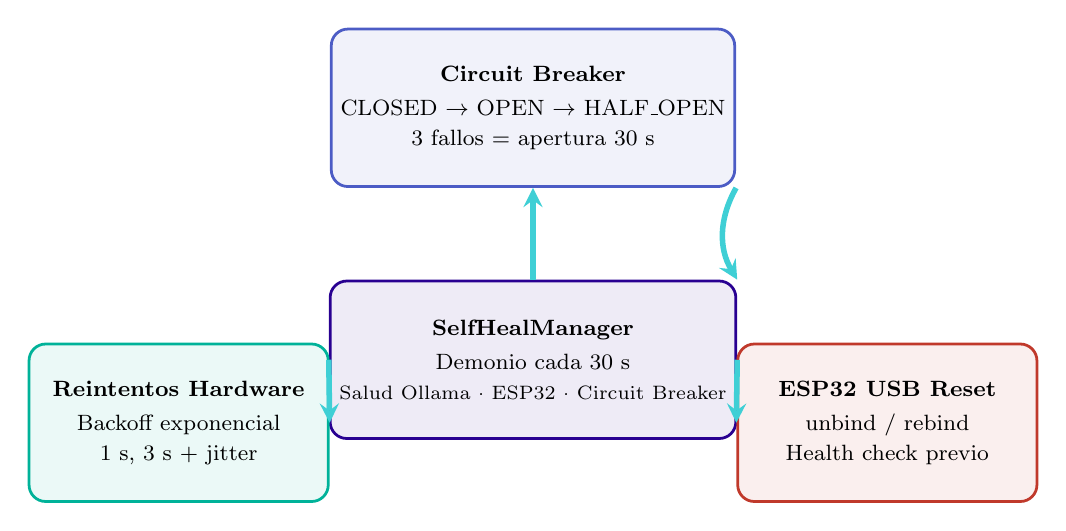
\begin{tikzpicture}[
    node/.style={draw=#1, fill=#1!8, rounded corners=6pt,
                 minimum width=3.8cm, minimum height=2cm, align=center,
                 font=\footnotesize, line width=1pt},
    arrow/.style={draw=accent, line width=2pt, ->, >=stealth, rounded corners=3pt},
]

% Centro: SelfHealManager
\node[node=primary] (self) at (0, 0) {
    \textbf{SelfHealManager}\\[0.1cm]
    Demonio cada 30 s\\[0.05cm]
    {\scriptsize Salud Ollama · ESP32 · Circuit Breaker}
};

% Superior: Circuit Breaker
\node[node=secondary] (cb) at (0, 3.2) {
    \textbf{Circuit Breaker}\\[0.1cm]
    CLOSED $\to$ OPEN $\to$ HALF\_OPEN\\[0.05cm]
    3 fallos = apertura 30 s
};

% Inferior izquierda: Reintentos
\node[node=exgreen] (retry) at (-4.5, -0.8) {
    \textbf{Reintentos Hardware}\\[0.1cm]
    Backoff exponencial\\[0.05cm]
    1 s, 3 s + jitter
};

% Inferior derecha: ESP32
\node[node=alertred] (esp32) at (4.5, -0.8) {
    \textbf{ESP32 USB Reset}\\[0.1cm]
    unbind / rebind\\[0.05cm]
    Health check previo
};

% Flechas
\draw[arrow] (self.north) -- (cb.south);
\draw[arrow] (self.west)  -- (retry.east);
\draw[arrow] (self.east)  -- (esp32.west);

% Bucle: CB -> Self
\draw[arrow, bend right=30] (cb.south east) to (self.north east);

\end{tikzpicture}
\end{document}
